\documentclass[conference]{IEEEtran}
\IEEEoverridecommandlockouts

\usepackage{cite}
\usepackage{amsmath,amssymb,amsfonts}
\usepackage{graphicx}
\usepackage{textcomp}
\usepackage{xcolor}
\usepackage{booktabs}

\def\BibTeX{{\rm B\kern-.05em{\sc i\kern-.025em b}\kern-.08em
    T\kern-.1667em\lower.7ex\hbox{E}\kern-.125emX}}

\begin{document}

\title{Classifier-Capacity Conditioning of the Quantum-Kernel Advantage in Rydberg-Atom DAQCNN}

\author{\IEEEauthorblockN{Anonymous Authors}}

\maketitle

\begin{abstract}
Recent work has applied digital-analog quantum convolutional neural networks
(DAQCNN) with neutral-atom Rydberg kernels to medical image classification.
We disentangle the design dimensions of the framework on two MedMNIST
datasets, BreastMNIST and PneumoniaMNIST: the encoding mode (digital versus
analog), the role of ZZ-correlator measurements, and the capacity of the
downstream trained classifier.
Across a five-tier head-capacity sweep on per-feature standardized inputs, the
strongest quantum source ties the strongest dimension-matched classical source
at every head on both datasets (best-quantum minus best-classical AUC within
$\pm 0.008$, inside one standard deviation).
The quantum kernels lead a \emph{linear} random projection at intermediate
capacity, but two classical nonlinear feature maps of equal dimensionality, a
degree-two polynomial and random Fourier features, reproduce that lead, and it
converges to a tie under a trained CNN.
The DAQCNN advantage in this regime is therefore conditional on classifier
capacity and attributable to nonlinear feature expansion rather than to quantum
structure.
The value of the ZZ correlators is in turn conditional on task structure: they
add $+0.025$ to $+0.040$ AUC over single-qubit $\langle Z\rangle$ marginals on
BreastMNIST, whose single-qubit features are only weakly separable, but are
negligible or mildly harmful on PneumoniaMNIST, which is already near-linearly
separable from $\langle Z\rangle$ alone.
Analog and digital encodings produce features of comparable linear
separability on both tasks, with mean encoding effects within one standard
deviation of zero across topologies.
At the trained-head operating point the best quantum and best
dimension-matched classical models reach parity on both datasets (AUC gaps of
$+0.006$, within one standard deviation).
\end{abstract}

\begin{IEEEkeywords}
Quantum machine learning, quantum kernels, Rydberg atoms, neutral-atom
processors, medical image classification, feature learning
\end{IEEEkeywords}


\section{Introduction}
\label{sec:introduction}

Quantum machine learning (QML) proposes using quantum circuits as feature maps,
exploiting entanglement and superposition to access high-dimensional
representations of classical data~\cite{biamonte2017quantum,havlicek2019supervised}.
Near-term neutral-atom processors are particularly attractive in this context:
programmable Rydberg atom arrays realise strongly-correlated many-body dynamics
whose native interactions couple qubits through physical proximity, offering a
path to quantum feature extraction without deep gate
circuits~\cite{browaeys2020many}.

Simen et al.~\cite{simen2024digital} formalised this opportunity as the
Digital-Analog Quantum Convolutional Neural Network (DAQCNN): non-trainable
neutral-atom quantum kernels, governed by native Ising interactions, slide
over image patches, extracting features that a classical CNN head learns to
classify.
Applied to BreastMNIST and PneumoniaMNIST~\cite{yang2023medmnist}, their model
matches or exceeds classical counterparts with a significantly reduced parameter
count.

Three design dimensions of this framework remain unexamined.
First, data can be encoded \emph{digitally} (as single-qubit rotations applied
before Hamiltonian evolution) or \emph{in analog form} (where pixel values modulate
per-atom detuning parameters, causing the data to drive the quantum dynamics
directly rather than merely prepare the initial state).
While local detuning has recently been shown to enhance the expressiveness of
neutral-atom Rydberg kernels on graph-structured data~\cite{djellabi2025attributed},
no systematic comparison of the two encoding modes at matched topology and
dimensionality on image data exists.
Second, pairwise ZZ correlators $\langle Z_i Z_j\rangle$, which capture
inter-qubit correlations induced by the entangling evolution, have not been
ablated against single-qubit expectations $\langle Z_i\rangle$ alone.
Third, the representational quality of the frozen quantum features has not been
assessed independently of the trained classification head.

We address all three questions and, as our central contribution, reframe them
around a fourth.
Using the DAQCNN framework with a van der Waals Rydberg Hamiltonian
($V_{ij} = C_6/r_{ij}^6$), we show that the DAQCNN quantum-kernel advantage is
conditional on the capacity of the downstream classifier: at matched
dimensionality it is sizable under a linear probe and shrinks as head capacity
grows, vanishing and slightly reversing under a trained convolutional head.
We establish this with a controlled five-tier head-capacity sweep, from a
linear probe to a trained convolutional head, applied to identical frozen
quantum features, and replicate it on two MedMNIST datasets.
We support it with two ablations.
First, linear probing identifies the pairwise ZZ correlators as the
load-bearing ingredient of the feature map on BreastMNIST, adding $+0.025$ to
$+0.040$ AUC over single-qubit $\langle Z\rangle$ marginals; their value is
itself conditional on task structure, however, falling to negligible or
negative on PneumoniaMNIST, whose images are already near-linearly separable
from single-qubit marginals alone.
Digital and analog encodings produce features of comparable linear separability
on both tasks.
Second, against dimension-matched random-projection baselines, no quantum
variant outperforms the classical baseline by more than one standard deviation
once an expressive trained head is added, on either dataset.
Experiments are conducted on BreastMNIST and
PneumoniaMNIST~\cite{yang2023medmnist} with ten-seed multi-run evaluation.


\section{Background}
\label{sec:background}

\subsection{Rydberg Hamiltonian}

The Rydberg atom Hamiltonian governing our quantum feature extractor is

\begin{equation}
  H(t) = \frac{\Omega(t)}{2}\sum_i \sigma_i^x
         - \Delta(t)\sum_i n_i
         + \sum_{i<j} V_{ij}\, n_i n_j ,
  \label{eq:rydberg}
\end{equation}

where $\sigma_i^x$ is the Pauli-$X$ operator on atom $i$,
$n_i = (I - Z_i)/2$ is the Rydberg occupation number operator,
$\Omega(t)$ and $\Delta(t)$ are the time-dependent global Rabi frequency and
detuning, and $V_{ij} = C_6/r_{ij}^6$ is the van der Waals interaction between
atoms $i$ and $j$ at separation $r_{ij}$~\cite{browaeys2020many}.
Because $V_{ij}$ decays as the sixth power of distance, only nearby atoms are
appreciably coupled; the interaction graph is therefore determined by the
physical layout of the atom array.

\paragraph{Digital encoding.}
Pixel values are encoded into initial single-qubit states via a fixed rotation
circuit applied to each qubit before Hamiltonian evolution.
The data enters only through the initial state; the subsequent dynamics are
pixel-independent.

\paragraph{Analog encoding.}
Each pixel $x_k$ contributes an additional per-atom detuning term $x_k n_k$
to~\eqref{eq:rydberg}, so the effective local detuning for atom $k$ becomes
$\Delta_{\mathrm{eff},k}(t) = \Delta(t) - x_k$.
The data modulates the Hamiltonian dynamics directly, producing pixel-dependent
quantum trajectories that differ qualitatively from the digital case.

After evolution for time $T$, we measure single-qubit expectations
$\langle Z_i\rangle$ for all $i$ and, when ZZ correlators are enabled,
all pairwise $\langle Z_iZ_j\rangle$.
For a $3\!\times\!3$ patch ($k^2=9$ qubits) this yields 9~or
$9 + \binom{9}{2} = 45$ features per kernel.

\subsection{Quantum Kernels for Classical Data}

Using a fixed quantum circuit as a feature map, embedding classical inputs
into measurement outcome vectors, is a general strategy for constructing
structured, high-dimensional representations~\cite{havlicek2019supervised}.
Whether such maps provide a practical advantage over classical alternatives
depends on the data distribution and the geometry of the induced
kernel~\cite{huang2021power}.
On neutral-atom platforms specifically, the quantum evolution kernel encodes
the input directly in the Rydberg Hamiltonian and reads out observables after
time evolution~\cite{henry2021quantum}, a construction closely related to the
analog encoding we study.

In the DAQCNN framework~\cite{simen2024digital}, and in our work, quantum
kernels are \emph{non-trainable}: Hamiltonian parameters are fixed before any
data is seen and no gradients are computed through the quantum layer.
Only the downstream classical head is trained by gradient descent.
This sidesteps the training instabilities associated with deep parameterised
quantum circuits and makes the quantum front-end fully reproducible across runs.

\subsection{MedMNIST}

MedMNIST v2~\cite{yang2023medmnist} is a standardised collection of
$28\!\times\!28$ medical image benchmarks with fixed train/validation/test
splits.
We evaluate on two binary benchmarks: BreastMNIST (breast ultrasound) and
PneumoniaMNIST (paediatric chest X-ray); all images are processed in
grayscale.


\section{Method}
\label{sec:method}

\subsection{Pipeline Overview}

Our model is a two-stage pipeline. In the first stage, a frozen quantum
convolutional layer extracts patch-level features from the input image; its
parameters are fixed before training begins and no gradients pass through it.
In the second stage, a lightweight classical CNN head is trained on these
features by gradient descent.
This separation keeps the quantum front-end fully reproducible across runs and
avoids the trainability problems associated with deep parameterised quantum
circuits.

\subsection{Quantum Feature Extraction}

\subsubsection{Patch preparation}

Input images ($28\!\times\!28$, grayscale) are first rescaled to
$[0,\pi]$ via per-image min--max normalisation, then partitioned by a
sliding window of size $k\!\times\!k$ with stride $s$, yielding
$(\lfloor(28-k)/s\rfloor + 1)^2$ patches of $k^2$ pixel values each.
Patch values inherit the per-image normalisation; we do not rescale
again within a patch.

\subsubsection{Encoding modes}

We evaluate two strategies for embedding pixel values into the quantum system.

\paragraph{Digital encoding.}
Each pixel $x_i$ is mapped to qubit $i$ via an $R_Y(x_i)$ rotation followed by
a Hadamard gate, preparing the product state
$|\psi_0\rangle = \bigotimes_{i=1}^{k^2} H\,R_Y(x_i)|0\rangle$ before
evolution.
The data enters only through the initial state; the subsequent dynamics are
data-independent.

\paragraph{Analog encoding.}
No state-preparation gates are applied.
Instead, each pixel $x_i$ is supplied as the local detuning of atom $i$,
modifying the Hamiltonian of Eq.~\eqref{eq:rydberg} to
\begin{equation}
  H_\mathrm{an}(t) = \frac{\Omega(t)}{2}\sum_i\sigma_i^x
    - \sum_i\bigl[\Delta(t) - x_i\bigr]n_i
    + \sum_{i<j}V_{ij}\,n_i n_j.
  \label{eq:analog}
\end{equation}
The state begins in $|0\rangle^{\otimes k^2}$ and the pixels drive the
quantum dynamics throughout the full evolution, producing
data-dependent quantum trajectories rather than a data-dependent initial state.

\subsubsection{Theoretical motivation for analog encoding}

Schuld, Sweke and Meyer~\cite{schuld2021encoding} characterise quantum
circuits with separable encoding blocks of \emph{fixed} generators
$\{H_i\}$ as partial Fourier series,
\begin{equation}
  f(\boldsymbol{x}) = \sum_{\omega \in \mathcal{F}} c_\omega(\boldsymbol{\theta})\,
                      e^{i\omega \cdot \boldsymbol{x}},
  \label{eq:fourier}
\end{equation}
with frequency set $\mathcal{F}$ fixed by the eigenvalue differences of
$\{H_i\}$ and Fourier coefficients $c_\omega(\boldsymbol{\theta})$
shaped by the trainable blocks.
Digital encoding fits this form: $R_Y(x_i) = e^{-ix_i\sigma_y/2}$ has
eigenvalues $\pm\tfrac{1}{2}$, restricting each pixel to the frequency
set $\{-1, 0, +1\}$, a degree-1 ceiling that training cannot raise.
In its exact-evolution limit, analog encoding falls outside this
characterisation because its generator
$H(\boldsymbol{x}) = H_0 + \sum_i x_i n_i$ is itself data-dependent.
The competition between the Rabi drive and the local detuning produces
an eigenvalue splitting
${\propto}\sqrt{\Omega^2+(\Delta-x_i)^2}$ that depends nonlinearly on
$x_i$, so the continuous-time propagator $e^{-iH(\boldsymbol{x})T}$ is
not a finite Fourier series in $\boldsymbol{x}$.
The first-order Trotterisation we actually implement reintroduces the
data through repeated factors $e^{-i x_i n_i\,\delta t}$ whose generator
$n_i$ is \emph{fixed}; by the same characterisation this realises a
finite Fourier series whose degree grows with the number of Trotter
steps.
In either case the accessible Fourier degree lies far above the
digital degree-one ceiling, which no choice of evolution can raise.
Many-qubit van der Waals interactions further introduce joint pixel-pair
dependencies that appear in the ZZ correlator outputs.
Consistent with this picture, local detuning has been shown both analytically
and empirically to increase the expressiveness of neutral-atom Rydberg kernels
on graph data~\cite{djellabi2025attributed}.
The two encodings therefore access qualitatively different function
classes; whether this distinction translates into a measurable
classification advantage on our datasets is an empirical question we
report on in Section~\ref{sec:results}.

\subsubsection{Hamiltonian evolution}

The global Rabi frequency and detuning ramp linearly in time,
$\Omega(t)=\Omega_0 t$ and $\Delta(t)=\Delta_0 t$,
with $\Omega_0=\Delta_0=1$ in our chosen units and evolution time fixed
at $T=2.5$.
The unitary is approximated by a first-order Trotterisation with step size
$\delta t=0.05$ ($50$ Trotter steps for $T=2.5$): the Hamiltonian is held
constant over each interval $[m\,\delta t,\,(m{+}1)\delta t]$ and the
product $e^{-iH(m\,\delta t)\,\delta t}$ is applied sequentially via
\texttt{qml.ApproxTimeEvolution}.

\subsubsection{Measurements and feature dimensionality}

After evolution we measure the expectation values $\langle Z_i\rangle$ for all
$k^2$ qubits.
When ZZ correlators are enabled, we additionally measure all pairwise
$\langle Z_i Z_j\rangle$.
The two-body observables $\langle Z_i Z_j\rangle$ carry information about
inter-qubit correlations that the single-qubit marginals do not capture:
for a product state $\langle Z_i Z_j\rangle = \langle Z_i\rangle\langle Z_j\rangle$
always holds, whereas entangling dynamics can break this equality.
Including ZZ correlators extends the feature space from $k^2$ to
$k^2 + \binom{k^2}{2}$ dimensions.
For a $3\!\times\!3$ kernel this yields 9 (Z-only) or 45 (Z+ZZ) features per
topology.
We perform a controlled ablation of Z-only versus Z+ZZ to isolate the
contribution of the entanglement-mediated correlators.

\subsection{Atom-Array Topologies}
\label{sec:topologies}

The interaction graph is determined by the physical positions of atoms, which
fix the pairwise distances $r_{ij}$ and hence the couplings
$V_{ij}=C_6/r_{ij}^6$.
We evaluate eight geometries for the $3\!\times\!3$ kernel:
\emph{kings} (full $3\!\times\!3$ grid at unit spacing);
\emph{horizontal} (three independent rows);
\emph{vertical} (three independent columns);
\emph{cross} (centre plus four cardinal neighbours, corners isolated);
\emph{ring} (perimeter atoms, centre removed);
\emph{chain} (nine atoms in a line);
\emph{star} (central hub connected to eight spokes);
and \emph{grid} ($3\!\times\!3$ grid at $1.5\times$ the unit spacing,
weakening all couplings and making nearest-neighbour interactions
dominate over diagonals in absolute terms).
Each topology defines a distinct entanglement structure and hence a distinct
feature map.
When $M$ topologies are used simultaneously, their feature vectors are
concatenated, yielding $M \times f_k$ features per patch where $f_k$ is the
per-topology feature count.

\subsection{Linear Feature Probing}
\label{sec:probing_method}

To assess representational quality independently of the trained head, we probe
frozen quantum feature maps with a linear classifier.
For each configuration, the spatial feature tensor
$(N,\,Mf_k,\,H_\mathrm{out},\,W_\mathrm{out})$ is flattened to
$(N,\,Mf_k\cdot H_\mathrm{out}\cdot W_\mathrm{out})$, standardised using a
\texttt{StandardScaler} fit on the training split only, and passed to a
\texttt{LinearSVC} ($C\!=\!1$).
AUC is computed from the raw decision-function scores (binary: standard AUROC;
multiclass: macro one-vs-rest).
Using a linear classifier is essential: a nonlinear probe would introduce its
own kernel and conflate the probe's representational power with that of the
quantum features.

Two baselines accompany each quantum variant.
\emph{Raw pixels}: the flattened image (784 values) with no feature extraction.
\emph{Random filters}: $N$ Gaussian random $k\!\times\!k$ filters (same stride,
$N$ matched to the quantum feature count per patch) applied to the raw image.
The random-filter baseline isolates whether the quantum interaction structure
contributes over unstructured projections of identical dimensionality.

The primary comparison is Digital-ZZ versus Analog-ZZ at matched
dimensionality, the same measurement set, and the same topology, which
isolates the encoding contribution from topology effects.
Because the per-topology encoding effect can change sign across
topologies, we sweep all eight $3\!\times\!3$ topologies and report the
encoding effect across them rather than relying on a single representative
choice.
Comparisons involving Z-only features differ in dimensionality and are
treated as indicative.

\subsection{Classical Head}
\label{sec:classical_head}

The quantum convolutional layer produces a spatial feature tensor of shape
$(B,\,Mf_k,\,h_\mathrm{out},\,w_\mathrm{out})$.
This is passed to a fixed-architecture head:
Conv$(64,2\!\times\!2)$--BN--Act--MaxPool$(2\!\times\!2)$--Conv$(64,2\!\times\!2)$--Act--Dropout--Flatten--Dropout--Linear$(C)$,
where Act is ReLU or GELU (selected by HP search) and $C$ is the number of
classes.
Only the head parameters carry gradients; the quantum layer is executed with
\texttt{diff\_method=None}, enforcing that no gradient is computed through
the quantum circuit.
Hyperparameters (learning rate, weight decay, gradient clipping, dropout,
activation, batch size, early-stopping patience, and cosine learning-rate
scheduler toggle) are tuned per model using Optuna~\cite{akiba2019optuna}
with validation accuracy as the objective; the test set is not accessed
during search.
For quantum models, the atom-array topology (the per-kernel choice from
the eight $3\!\times\!3$ geometries, or a four-topology subset at the
multi-kernel scale) is included in the Optuna search space alongside the
training hyperparameters.

\subsection{Head-Capacity Sweep}
\label{sec:method_capacity}

To test whether the quantum-versus-classical advantage depends on the
expressivity of the trained classifier, we vary the head architecture
while keeping the frozen feature substrate fixed.
We evaluate five head capacities of increasing expressivity, ordered by
architectural expressivity:
\begin{itemize}
\item \emph{Linear}: \texttt{Flatten} + \texttt{Linear}$(C)$.
\item \emph{MLP-1}: \texttt{Flatten} + \texttt{Linear}$(H)$ + Act + Dropout
        + \texttt{Linear}$(C)$, with $H=32$.
\item \emph{MLP-2}: \texttt{Flatten} + \texttt{Linear}$(H_1)$ + Act + Dropout
        + \texttt{Linear}$(H_2)$ + Act + Dropout + \texttt{Linear}$(C)$,
        with $H_1=64,\,H_2=32$.
\item \emph{CNN-16}: the classification head of
        Section~\ref{sec:classical_head} with $16$ channels in the
        convolutional stack.
\item \emph{CNN-64}: the same head with $64$ channels (the default used
        elsewhere in this work).
\end{itemize}

For each (head, feature source) cell, a 30-trial Optuna search over
learning rate, weight decay, and dropout selects the best
configuration on validation accuracy; the top-$1$ configuration is then
validated over $10$ random seeds.
All other training settings (Adam optimiser, cosine learning-rate
schedule, gradient clipping, batch size, early-stopping patience) are
fixed to the same values across cells.
Feature sources span both scales: at $M=1$ we use the best-performing
topology of each encoding mode from Section~\ref{sec:probing_method},
matched in dimensionality ($3{,}645$ features per patch) against a
classical Random$\times 45$ baseline; at $M=4$ we use the
four-topology set found by Optuna for each encoding, matched at
$14{,}580$ features per patch against Random$\times 180$.
All feature sources are per-feature standardized (mean and variance fit
on the training split, applied to validation and test) before the head,
so the comparison reflects information content rather than the differing
magnitudes of the quantum, random, and nonlinear maps.
We further include three classical nonlinear controls operating on the
same raw image patches as the random baseline: a per-patch degree-two
polynomial map (poly-2, the nine pixels and their $36$ pairwise products,
$45$ features, a structural match to $\langle Z\rangle$ plus
$\langle ZZ\rangle$) and random Fourier features approximating an RBF
kernel at $45$ and $180$ dimensions (RFF).
These isolate whether any low-capacity advantage requires the quantum
kernel or follows from nonlinear feature expansion alone.
Because each cell tunes only learning rate, weight decay, and dropout at
a fixed topology, the absolute AUCs in this sweep are not directly
comparable to the full-search operating points of
Table~\ref{tab:endtoend}; the sweep is designed to expose the trend
across head capacity rather than to reproduce those values.


\section{Experimental Setup}
\label{sec:experiments}

\subsection{Datasets}

We evaluate on two binary MedMNIST v2~\cite{yang2023medmnist} datasets, both
$2$-class and processed in grayscale at $28\!\times\!28$.
\emph{BreastMNIST}: breast-ultrasound images, $546/78/156$ train/val/test
split.
\emph{PneumoniaMNIST}: paediatric chest-X-ray images, $4708/524/624$ split.
The two differ markedly in size and in how separable they are from simple
features, which is central to the task-structure effect we report.

\subsection{Models}

We evaluate six model families.
The three DAQCNN variants are run at single-kernel ($M\!=\!1$) and, where
indicated, four-kernel ($M\!=\!4$) scales.
\emph{DAQCNN-Digital-Z}: digital encoding, $\langle Z\rangle$ only, following
Simen et al.~\cite{simen2024digital}.
\emph{DAQCNN-Digital-ZZ}: digital encoding with ZZ correlators.
\emph{DAQCNN-Analog-ZZ}: analog encoding with ZZ correlators.
\emph{Classical-Random}: fixed Gaussian random $3\!\times\!3$ filters, channel
count matched to the corresponding quantum variant.
\emph{Classical-Trainable}: same architecture with learned filters.
\emph{Raw-pixel baseline}: the classification head applied to flattened
raw pixel values, with no front-end feature extraction.
All models share the same classification head architecture and are trained
under identical conditions.

\subsection{Hyperparameter Search and Evaluation}

Hyperparameters are tuned independently for each model using
Optuna~\cite{akiba2019optuna} (TPE sampler, 200 trials per search).
The objective is validation accuracy; the test set is not accessed during
search.
For quantum models, atom-array topology is included in the search space
alongside training hyperparameters, which means quantum models face a strictly
harder search problem than classical models under the same trial budget.
The top-1 configuration from each search is re-evaluated over ten random seeds;
we report mean $\pm$ standard deviation of test accuracy and AUC.

\subsection{Implementation}

Quantum circuits are implemented in PennyLane~\cite{bergholm2018pennylane} with
Trotterised time evolution ($\delta t\!=\!0.05$).
Features are pre-computed and cached before training; only the classical head
incurs per-epoch cost.
Experiments run on a single workstation CPU; cached features make full
training and hyperparameter search tractable without dedicated GPU
hardware.


\section{Results}
\label{sec:results}

% Numbers in this section are all derived from primary output files
% under outputs/paper_results/. Verified end-to-end (10-seed validation
% JSONs), capacity-sweep summary.csv, and topology-sweep CSV before
% writing. Do not edit numbers without re-verifying against those files.

\subsection{Linear Feature Probing}
\label{sec:results_probing}

Figure~\ref{fig:topology_probing} reports the linear-SVM probing AUC
for all eight $3\!\times\!3$ topologies of each encoding mode at the
single-kernel scale, and for five four-topology sets at the four-kernel
scale.

\begin{figure}[t]
\centering
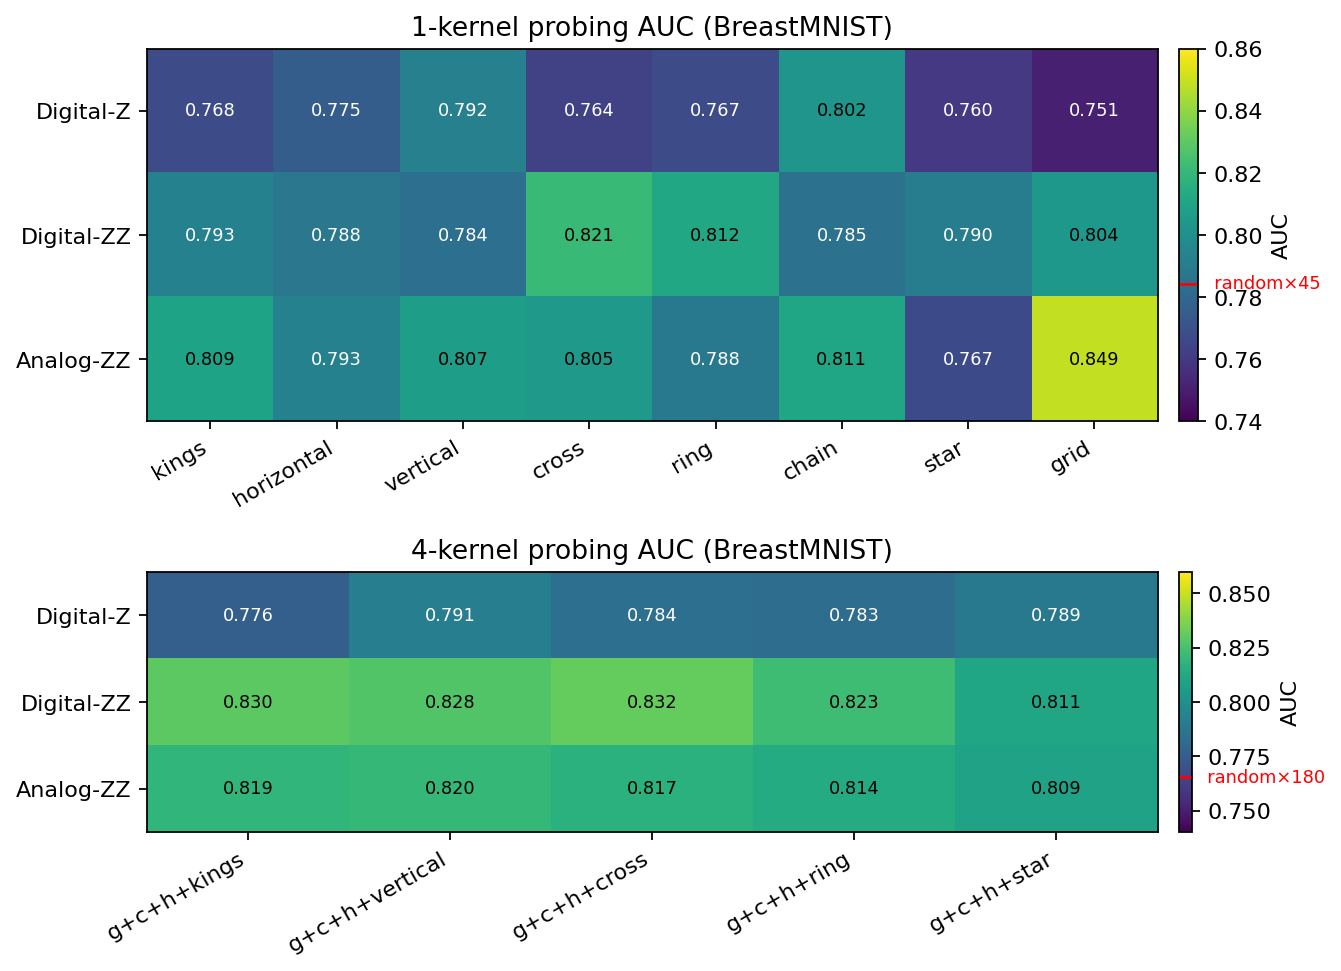
\includegraphics[width=\columnwidth]{figures/topology_sweep_heatmap.pdf}
\caption{Linear-SVM probing AUC on BreastMNIST.
\emph{Top}: eight $3\!\times\!3$ topologies $\times$ three encoding
modes at single-kernel scale ($3{,}645$-dim, except Digital-Z at
$729$).
\emph{Bottom}: five four-topology sets $\times$ three encodings at
four-kernel scale ($14{,}580$-dim, except Digital-Z at $2{,}916$).
The red line on each colourbar marks the dimension-matched random
projection baseline.}
\label{fig:topology_probing}
\end{figure}

On BreastMNIST, at matched dimensionality ($3{,}645$ features), quantum
kernels with ZZ correlators outperform classical random projections on
every topology tested.
The mean probing AUC across the eight $3\!\times\!3$ topologies is
$0.797$ for Digital-ZZ and $0.804$ for Analog-ZZ, against $0.766$ for
the Random$\times 45$ baseline.
Digital-Z, which omits the ZZ correlator outputs, reaches a mean of
$0.772$, essentially matching the random-filter baseline: single-qubit
$\langle Z_i\rangle$ marginals on their own carry little separability
beyond what unstructured random projections
already span.

\paragraph{ZZ correlators.}
At matched topology and digital encoding, enabling ZZ correlators
raises probing AUC by a mean of $+0.025$ across the eight $3\!\times\!3$
topologies (range $-0.018$ to $+0.058$), with positive sign in six of
eight topologies.
The same ablation at the four-kernel scale yields a larger mean effect
of $+0.040$ (range $+0.022$ to $+0.054$), positive across all five
topology sets tested.
ZZ correlators carry information that the single-qubit marginals do
not, consistent with their interpretation as observables of
inter-qubit correlations induced by entangling dynamics.

\paragraph{Encoding mode.}
At matched topology and matched measurement set, the encoding effect
is small and topology-dependent.
The mean of $(\mathrm{Analog\text{-}ZZ}) - (\mathrm{Digital\text{-}ZZ})$
across the eight $3\!\times\!3$ topologies is $+0.007$ AUC (analog
wins five of eight topologies), and the same statistic at the
four-kernel scale is $-0.009$ AUC (digital wins all five sets).
Both means are within one standard deviation of zero across topologies.
The two encodings access qualitatively different function classes
(Section~\ref{sec:method}), but on BreastMNIST they produce features
of comparable linear separability.

\paragraph{Task-structure dependence (PneumoniaMNIST).}
The picture changes on PneumoniaMNIST, whose images are already
highly separable from single-qubit features.
The mean Digital-Z probing AUC across the eight $3\!\times\!3$ topologies
is $0.923$ (best $0.934$, \emph{vertical}), against $0.772$ on BreastMNIST.
With little separability headroom left, the ZZ correlators add almost
nothing: the Digital-ZZ$-$Digital-Z effect is only $+0.003$ at single-kernel
scale (positive in six of eight topologies) and turns \emph{negative} at
four-kernel scale ($-0.013$ digital, $-0.021$ analog), where the additional
correlator dimensions act as noise rather than signal.
The encoding effect is again small (mean
$(\mathrm{Analog\text{-}ZZ})-(\mathrm{Digital\text{-}ZZ})$ of $-0.012$ at
single-kernel scale).
The load-bearing role of the ZZ correlators is therefore specific to tasks,
like BreastMNIST, whose single-qubit representation leaves separability
headroom; on a task already near-linearly separable from $\langle Z\rangle$
alone, the correlators are redundant.

\subsection{End-to-End Classification}
\label{sec:results_endtoend}

\begin{table}[t]
\centering
\caption{End-to-end test classification on BreastMNIST.
Mean $\pm$ standard deviation over $10$ random seeds.
Hyperparameters are independently tuned per model with Optuna
($200$ trials, validation accuracy as objective).
For quantum models the winning topology is in parentheses;
four-kernel sets all include \emph{grid}, \emph{chain}, and
\emph{horizontal}, with the fourth topology shown after $+$.}
\label{tab:endtoend}
\begin{tabular}{lcc}
\toprule
Model & Acc & AUC \\
\midrule
\multicolumn{3}{l}{\emph{Quantum (DAQCNN)}} \\
Digital-Z 1k (\emph{ring}) & $0.848 \pm 0.018$ & $0.868 \pm 0.007$ \\
Digital-ZZ 1k (\emph{cross}) & $0.855 \pm 0.016$ & $0.883 \pm 0.012$ \\
Analog-ZZ 1k (\emph{star}) & $0.844 \pm 0.009$ & $0.889 \pm 0.010$ \\
Digital-ZZ 4k ($+$\emph{ring}) & $0.852 \pm 0.016$ & $\mathbf{0.901 \pm 0.005}$ \\
Analog-ZZ 4k ($+$\emph{kings}) & $0.847 \pm 0.018$ & $0.893 \pm 0.010$ \\
\midrule
\multicolumn{3}{l}{\emph{Classical}} \\
Random $\times 45$    & $\mathbf{0.862 \pm 0.007}$ & $0.895 \pm 0.010$ \\
Trainable $\times 45$ & $\mathbf{0.862 \pm 0.013}$ & $0.889 \pm 0.015$ \\
Random $\times 180$   & $0.858 \pm 0.014$ & $0.893 \pm 0.009$ \\
Trainable $\times 180$ & $0.835 \pm 0.029$ & $0.863 \pm 0.016$ \\
\midrule
\multicolumn{3}{l}{\emph{Baseline}} \\
Raw pixels  & $0.824 \pm 0.010$ & $0.843 \pm 0.004$ \\
\bottomrule
\end{tabular}
\end{table}

Table~\ref{tab:endtoend} reports test accuracy and AUC for the seven
model families after $10$-seed validation of each Optuna top-$1$
configuration.

\paragraph{No family dominates.}
The highest AUC ($0.901 \pm 0.005$) is achieved by Digital-ZZ at the
four-kernel scale; the highest accuracy ($0.862$) is shared by
Classical-Random and Classical-Trainable at the single-kernel scale.
The best-quantum-vs-best-classical AUC gap is $+0.006$ in favour of
the quantum model; the corresponding accuracy gap is $+0.010$ in
favour of the classical model.
Both differences fall within one standard deviation.

\paragraph{ZZ ablation at end-to-end.}
At the single-kernel scale, Digital-Z reaches AUC $0.868 \pm 0.007$
and Digital-ZZ reaches $0.883 \pm 0.012$; including ZZ correlators
adds $+0.015$ AUC at the trained-head level, consistent in direction
with the probe-level finding although smaller in magnitude.

\paragraph{Encoding ablation at end-to-end.}
The single- and four-kernel scales disagree on which encoding wins,
both by under one standard deviation.
At $M=1$, Analog-ZZ achieves AUC $0.889 \pm 0.010$ versus Digital-ZZ's
$0.883 \pm 0.012$ ($+0.006$ for analog).
At $M=4$, Digital-ZZ achieves $0.901 \pm 0.005$ versus Analog-ZZ's
$0.893 \pm 0.010$ ($+0.008$ for digital).
The end-to-end encoding-effect direction therefore flips with
dimensionality, mirroring the same pattern seen in the topology
probing (Section~\ref{sec:results_probing}).

\begin{table}[t]
\centering
\caption{End-to-end test classification on PneumoniaMNIST.
Mean $\pm$ standard deviation over $10$ random seeds, same protocol as
Table~\ref{tab:endtoend}.
For quantum models the winning topology is in parentheses; both
four-kernel sets are \emph{grid}, \emph{chain}, \emph{horizontal}, and
\emph{kings} ($+$\emph{kings}).}
\label{tab:endtoend_pneumonia}
\begin{tabular}{lcc}
\toprule
Model & Acc & AUC \\
\midrule
\multicolumn{3}{l}{\emph{Quantum (DAQCNN)}} \\
Digital-Z 1k (\emph{cross}) & $0.865 \pm 0.007$ & $0.953 \pm 0.002$ \\
Digital-ZZ 1k (\emph{vertical}) & $0.858 \pm 0.006$ & $0.948 \pm 0.005$ \\
Analog-ZZ 1k (\emph{ring}) & $0.858 \pm 0.007$ & $0.943 \pm 0.004$ \\
Digital-ZZ 4k ($+$\emph{kings}) & $\mathbf{0.869 \pm 0.020}$ & $0.955 \pm 0.002$ \\
Analog-ZZ 4k ($+$\emph{kings}) & $0.859 \pm 0.008$ & $\mathbf{0.959 \pm 0.002}$ \\
\midrule
\multicolumn{3}{l}{\emph{Classical}} \\
Random $\times 45$    & $0.849 \pm 0.007$ & $0.952 \pm 0.003$ \\
Trainable $\times 45$ & $0.857 \pm 0.005$ & $0.950 \pm 0.002$ \\
Random $\times 180$   & $0.845 \pm 0.006$ & $0.953 \pm 0.003$ \\
Trainable $\times 180$ & $0.857 \pm 0.011$ & $0.945 \pm 0.004$ \\
\midrule
\multicolumn{3}{l}{\emph{Baseline}} \\
Raw pixels  & $0.855 \pm 0.005$ & $0.951 \pm 0.002$ \\
\bottomrule
\end{tabular}
\end{table}

\paragraph{Parity on PneumoniaMNIST.}
Table~\ref{tab:endtoend_pneumonia} repeats the evaluation on PneumoniaMNIST.
The highest AUC ($0.959 \pm 0.002$, Analog-ZZ at four-kernel scale) exceeds the
best dimension-matched classical model (Random$\times 180$, $0.953 \pm 0.003$)
by $+0.006$, within one standard deviation, the same parity margin found on
BreastMNIST.
Consistent with the probing analysis, ZZ correlators give no end-to-end
benefit here: at single-kernel scale Digital-Z ($0.953$) slightly exceeds
Digital-ZZ ($0.948$), and the strongest single-kernel model is the
correlator-free Analog-Z ($0.954$).
The dataset that gains from correlators at the probe (BreastMNIST) is also the
one where they survive to the operating point; the dataset that does not
(PneumoniaMNIST) shows no end-to-end ZZ benefit, reinforcing the
task-structure dependence of Section~\ref{sec:results_probing}.

\subsection{Head-Capacity Sweep}
\label{sec:results_capacity}

The previous two subsections establish that quantum kernels with ZZ
correlators are more linearly separable than dimension-matched random
projections (Section~\ref{sec:results_probing}), yet this advantage
does not propagate cleanly to the end-to-end accuracy table once a
trained CNN head is added (Section~\ref{sec:results_endtoend}).
The head-capacity sweep traces this gap directly as a function of head
expressivity.
All feature sources in this sweep are per-feature standardized
(z-scored on the training split) before the head, so the comparison
measures information content rather than feature scale.
We further add two classical nonlinear feature maps of matched
dimensionality, a per-patch degree-two polynomial expansion (poly-2,
$45$ features: nine pixels and their $36$ pairwise products, a
structural match to $\langle Z\rangle$ plus $\langle ZZ\rangle$) and
random Fourier features (RFF) at $45$ and $180$ dimensions, to test
whether any low-capacity advantage is specific to the quantum kernel or
is recovered by classical nonlinearity alone.

\begin{figure*}[t]
\centering
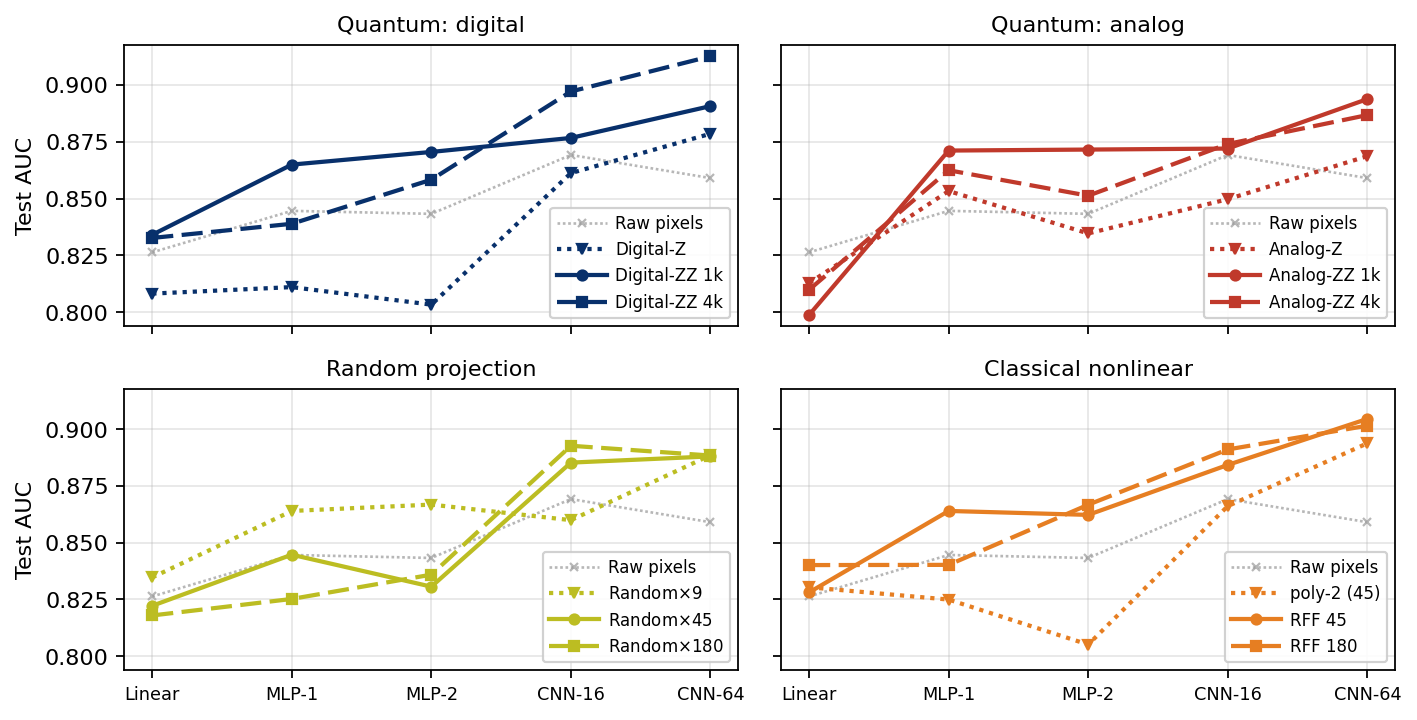
\includegraphics[width=\textwidth]{figures/capacity_sweep.pdf}
\caption{Test AUC on BreastMNIST as a function of head capacity, faceted
by feature family (quantum-digital, quantum-analog, random projection,
and classical nonlinear maps).
All panels share the $y$-axis, and raw pixels are drawn faintly in each
as a common cross-panel reference.
Within a panel, scale is encoded by both marker and line style: a
down-triangle on a dotted line is the single-qubit $\langle Z\rangle$-only
source ($9$ features per patch), a circle on a solid line is the
single-kernel $\langle ZZ\rangle$ source ($45$), and a square on a dashed
line is the four-kernel source ($180$). The random and classical-nonlinear
families reuse the same three styles for their $9$/$45$/$180$ and
$45$/$45$/$180$ variants, respectively.
Heads are ordered by expressivity from Linear to CNN-$64$; each point is
a $10$-seed mean over per-feature standardized inputs.
Every quantum and classical source converges to the same band as head
capacity grows.}
\label{fig:capacity_sweep}
\end{figure*}

\paragraph{Quantum versus classical nonlinearity.}
With features standardized, the strongest quantum source and the
strongest dimension-matched classical source track each other across
the entire ladder.
The best-quantum minus best-classical AUC difference stays within
$\pm 0.008$ at every head on both datasets (BreastMNIST: $-0.006$,
$+0.007$, $+0.005$, $+0.004$, $+0.008$ across the five heads;
PneumoniaMNIST: $-0.003$, $+0.006$, $+0.003$, $+0.003$, $-0.001$), all
inside one standard deviation.
The decisive control is the nonlinear map.
Digital-ZZ never exceeds RFF by more than one standard deviation at any
head on either dataset, and on PneumoniaMNIST RFF significantly
outperforms Digital-ZZ at the linear probe ($-0.030$) and at CNN-$16$
($-0.010$).
A classical degree-two polynomial and an RBF random-feature map of the
same dimensionality thus reproduce whatever the quantum kernel provides.

\paragraph{Quantum versus random projection, and capacity conditioning.}
Against the \emph{linear} random projection the quantum sources do lead
at intermediate capacity: the Digital-ZZ minus Random$\times 45$ gap is
$+0.020$ and $+0.040$ on BreastMNIST at MLP-$1$ and MLP-$2$, and
$+0.008$ and $+0.010$ on PneumoniaMNIST, each exceeding one standard
deviation.
But poly-2 and RFF achieve the same margin over the random projection,
so this lead reflects nonlinear feature expansion rather than quantum
structure, and it converges to within noise at the CNN heads.
The low-capacity behaviour is moreover dataset dependent.
On the near-linearly-separable PneumoniaMNIST the quantum sources are
the \emph{weakest} at the linear probe (Digital-ZZ $0.901$ at
single-kernel and $0.877$ at four-kernel scale, versus raw pixels
$0.932$, Random$\times 45$ $0.925$, and RFF $0.931$), as the entangling
transform disrupts structure that is already linearly accessible; only
on BreastMNIST, whose raw separability is lower, do the quantum sources
lead at the probe.

\paragraph{ZZ ablation across capacities.}
The benefit of the correlators is itself task dependent.
On BreastMNIST the Digital-ZZ minus Digital-Z gap is large and
significant at low capacity ($+0.026$, $+0.054$, $+0.067$ across Linear,
MLP-$1$, and MLP-$2$) and remains positive but within noise at the two
CNN heads ($+0.015$, $+0.012$).
On PneumoniaMNIST the same gap is negative at the probe ($-0.029$) and
small thereafter ($+0.009$, $+0.007$, $-0.004$, $+0.002$), consistent
with that task being already separable from $\langle Z\rangle$ alone.
The correlators add separable structure only when the single-qubit
representation leaves headroom.

\begin{figure*}[t]
\centering
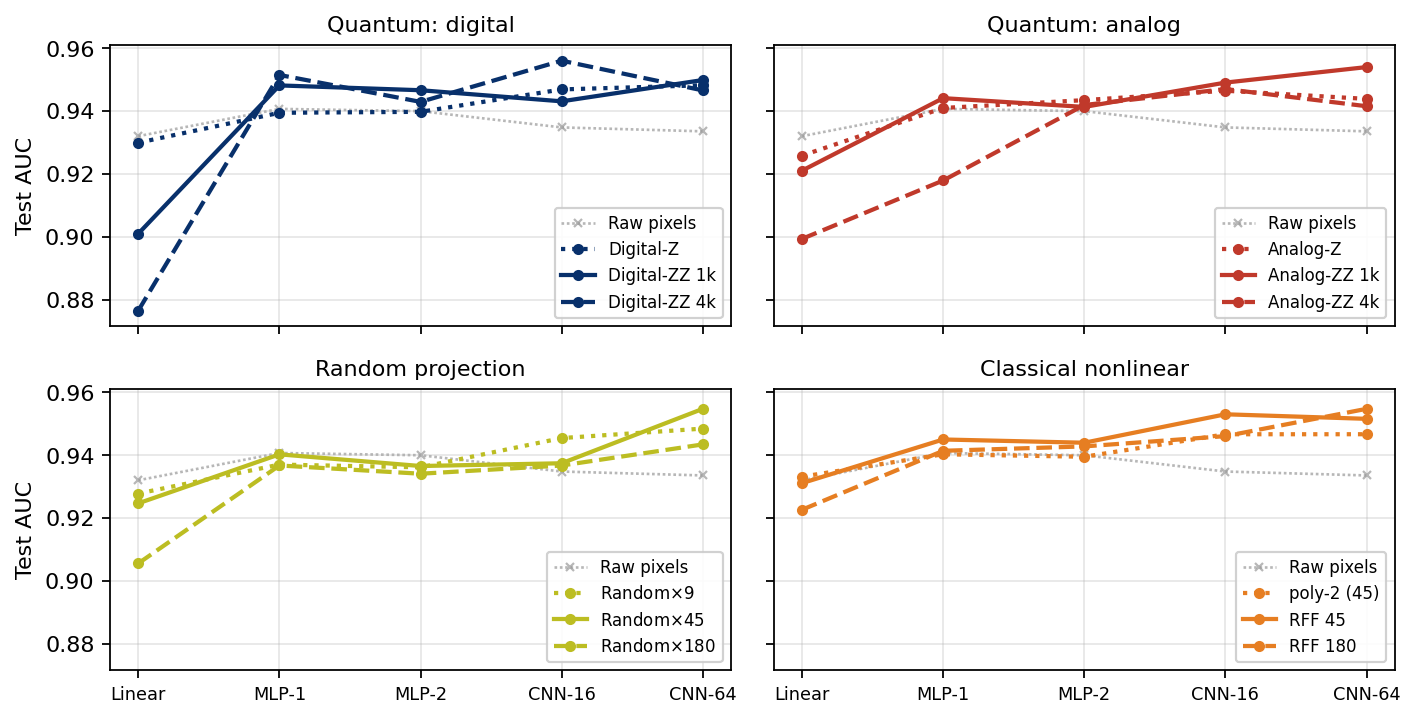
\includegraphics[width=\textwidth]{figures/capacity_sweep_pneumonia.pdf}
\caption{The same faceted head-capacity sweep on PneumoniaMNIST, with
identical panels, sources, and styling to Fig.~\ref{fig:capacity_sweep}.
Because this task is near-linearly separable from raw and simple
features, the quantum sources are the weakest at the linear probe and
converge to the classical nonlinear and random sources by the CNN
heads.}
\label{fig:capacity_pneumonia}
\end{figure*}

\paragraph{Cross-dataset summary
(Fig.~\ref{fig:capacity_pneumonia}).}
The two datasets agree on the central point and differ only in where the
low-capacity quantum lead appears.
On both, the best quantum source ties the best classical nonlinear map
at every head, and all feature substrates converge under the trained
CNN; the lead over the linear random projection at intermediate capacity
is reproduced by poly-2 and RFF.
They differ at the probe: BreastMNIST, with low raw separability, favours
the quantum sources there, whereas PneumoniaMNIST, already separable from
simple features, ranks them last.

\paragraph{Interpretation.}
The sweep isolates one effect, identifies its source, and shows what
gates it.
The low-capacity edge over a random projection is real but is reproduced
by classical nonlinear feature maps of equal dimension, so it is
attributable to nonlinear feature expansion rather than to quantum
structure: a degree-two polynomial of the same patch matches the quantum
kernel at every head.
That edge is gated by classifier capacity, shrinking to a tie once the
head is an expressive CNN, and by task structure, appearing only where
the single-qubit representation leaves separable headroom (BreastMNIST,
probe AUC $0.77$) and not where the task is already easy
(PneumoniaMNIST, probe AUC $0.92$).
A measurable quantum or ZZ advantage thus appears only when the head is
weak, the task is hard from simple features, and no matched classical
nonlinearity is in the comparison; relax any of these and it vanishes.


\section{Conclusion}
\label{sec:conclusion}

We evaluated DAQCNN-style Rydberg quantum kernels on BreastMNIST and
PneumoniaMNIST with methodologically clean per-model hyperparameter
searches, ten-seed validation, dimensionality-matched classical
baselines, and a controlled head-capacity sweep.
Three findings emerge.

\paragraph{The ZZ correlators are load-bearing, but only when the task
needs them.}
On BreastMNIST, single-qubit $\langle Z_i\rangle$ measurements alone
(Digital-Z) produce features whose linear separability is no better than
that of unstructured random projections (mean AUC $0.772$, versus
$0.766$ for the higher-dimensional Random$\times 45$ baseline), and
adding the pairwise $\langle Z_iZ_j\rangle$ correlators raises mean
probing AUC by $+0.025$ at single-kernel scale and $+0.040$ at
four-kernel scale.
On PneumoniaMNIST the single-qubit features are already highly separable
(Digital-Z probe AUC $0.923$), and the correlators add essentially
nothing ($+0.003$ at single-kernel scale, negative at four-kernel
scale).
The entanglement-mediated correlators help only when the single-qubit
representation leaves separability headroom.

\paragraph{The quantum-versus-classical advantage is conditional on
classifier capacity and is not specifically quantum.}
The quantum kernels lead a dimension-matched \emph{linear} random
projection at intermediate capacity, by up to $+0.040$ AUC on
BreastMNIST, but classical nonlinear feature maps of the same
dimensionality, a per-patch degree-two polynomial and random Fourier
features, reproduce that lead.
The strongest quantum source ties the strongest classical source at
every head on both datasets (best-quantum minus best-classical within
$\pm 0.008$, inside one standard deviation), and on the near-separable
PneumoniaMNIST the quantum sources are in fact the weakest at the linear
probe.
As classifier capacity grows the gap over the random projection shrinks
to a statistical tie under a trained CNN.
The DAQCNN advantage in this regime therefore lives at the feature
substrate, is reproduced by classical nonlinearity, and is absorbed by a
sufficiently expressive trained head.
This pattern is consistent with independent large-scale evidence on
neutral-atom hardware, where an analog quantum-reservoir advantage over
classical learners is observed only on synthetic datasets constructed to
exhibit a quantum-classical kernel separation, and not on natural
data~\cite{kornjaca2024largescale}.

\paragraph{Encoding mode is empirically neutral on these tasks.}
The qualitatively broader function class accessed by analog encoding
does not translate into a measurable classification advantage on either
dataset.
Although local detuning increases Rydberg-kernel expressiveness on
graph-structured data~\cite{djellabi2025attributed}, on image classification
at this resolution and dataset size that broader function class does not
improve linear separability.
We interpret this as a scope limitation rather than a refutation of
the framework: image classification at this resolution is not
bottlenecked by the Fourier ceiling of digital encoding,
since the target function is dominated by spatial texture and shape
structure that a degree-one Fourier basis on pixel intensities,
combined with entangling Hamiltonian dynamics, can already express.
Tasks whose target function depends on input values through
high-frequency or irrational-frequency components, such as
signal-processing problems, tabular regression with oscillatory
dependencies, or symbolic regression, may be more natural settings in
which the analog advantage manifests, and we leave such evaluation to
future work.
Extending this analysis to multi-class and higher-resolution MedMNIST
benchmarks, where single-qubit separability is lower and the capacity
and task-structure axes can be probed jointly, is a natural next step.

\paragraph{Tuning the quantum kernel.}
Our kernels are frozen at a single evolution time ($T = 2.5$) and fixed
atom geometries, so these results bound only the untuned configuration.
A natural next step is a joint sweep of evolution time and array
geometry under both encodings, paired with a direct measure of the
generated entanglement (bipartite von Neumann entropy) and of
kernel-target alignment, to test whether the usefulness of the feature
substrate is sensitive to these physical controls or saturates
regardless of them.
Such a sweep is a coarse, gradient-free form of kernel tuning, and a
prerequisite for the more ambitious direction of trainable Rydberg
kernels in which the detuning schedule or geometry is optimized end to
end.
We regard the latter as promising but contingent: it must contend with
the exponential-concentration barrier that limits the trainability of
generic quantum kernels, and our capacity-conditioning result suggests
that on tasks where classical nonlinear feature maps already saturate
performance, optimizing the kernel may yield little beyond a costlier
route to the same ceiling.
The strongest case for trainable kernels is therefore on data with an
intrinsic quantum-classical kernel separation rather than on natural
images at this scale.


\section*{Acknowledgment}


\bibliographystyle{IEEEtran}
\bibliography{references}

\end{document}
